\documentclass{article}
\usepackage[utf8]{inputenc}
\usepackage{graphicx}
\usepackage{hyperref}
\usepackage{tikz}
\usepackage{pgfplots}
\usepackage{graphicx}
\usepackage{subcaption}
\usepackage{indentfirst}
\usepackage{float}
\usepackage{tcolorbox}
\documentclass{article}
\usepackage{amsmath}

\definecolor{codegray}{gray}{0.9}
\newcommand{\code}[1]{\colorbox{codegray}{\texttt{#1}}}

\title{AG Tema 2 \& 2p}
\author{Stefan Petrovici}
\date{November 2019}

\pagestyle{empty}
\pgfplotsset{compat=1.16}
\begin{document}

\maketitle

\section{Introduction}
This report takes a closer look at what are the particularities of the genetic algorithms. We will firstly discuss general aspects, and then compare results of a genetic algorithm with our previously analyzed heuristic algorithms: Hillclimber and Simmulated Annealing. The three algorithms will try to solve the Minimization Problem on four functions(Rastrigin, Schwefel, Rosenbock and Sphere). These results will be represented by a number of comparative tables and graphs that will then allow us to obtain a conclusion about genetic algorithms.

\subsection{Problem}
If we look at some of the heuristic algorithms (HillClimbing, for instance) we will notice that while their approach is indeed one that is randomized, the way they tackle finding the optimum is rather by trying out sistematic changes to our current solution. This is a great improvement from the deterministic way of doing things, of course, because now we don't have to consume a large amount of resources to compute the output to our problem. But if these algorithms have a small part that resemble deterministic methods, could we go even further and randomize the process more? The answer is yes, by using genetic algorithms. By having a fully-heuristic way to search for a solution we now start to analyze its different parameters and particularities, and how each influences the final solution.

\clearpage

\section{Method}
\subsection{Pseudocode}

The pseudocode for GA is shown below:

\begin{tcolorbox}
begin\\
t := 0\\
generate P(t)\\
evaluate P(t)\\
\ \ while (not STOP\_CONDITION()) do begin: \\
\ \ mutate P(t)\\
\ \ crossover P(t)\\
\ \ select P(t + 1) from P(t)\\
\ \ t := t + 1\\
end
\end{tcolorbox}

\subsection{Description}
Genetic algorithms resemble the HC and SA algorithms, and that is obvious when we look at their structure. We have the initialization and a loop in which we modify the candidates slightly and compare them.

The representation for the solution to this problem is a bitstring that represents a real number in the interval of the chosen function.

In the initialization part we have to choose a random solution, and for that we give each gene a probability of 50\% of choosing each of the two possible values. We choose this probability as an assurance that whatever problem we have, we can start closer to it by initializing values that are (virtually) in the middle area.

\subsection{The particularities of the GA algorithm}
The algorithm consists in three major procedures: mutation, crossover and selection.

\subsection{Mutation}
The mutation procedure allows every gene in a chromosome to change, though this chance is small (1\%). The mutation gene comes first in this algorithm because it is the only procedure that actually changes the information that the population carries. We can see that in a test with no mutation the variation from one population to another is slower than that in a normal run, and that could be explained like this: if we imagine the “optimal” genes that the chromosomes are carrying as units on a distribution graph, the overall “optimality” of the population does not actually change, as the number of good genes do not change in the crossover or selection procedure. Only by mutation it is that we ca gain optimal genes and thus changing the distribution. To offer an example in which we can identify these optimal genes we can look at the minimization problem of the Rastrigin function: in this case the global minimum is 0.0, thus the optimal genes we are looking for are the ones that have a numeric value of 0. \\\\
\par While it is true that we can talk about optimal genes only when they are in combination with the other genes, it is also a fact that the “winning” chromosome has a range of neighbors that resemble its particular “distribution” that we have talked earlier. So we can approach the optimal solution by matching its number of favorable genes.

\subsection{Implementation of mutation}
The standard method for mutating chromosomes is to give each individual gene a chance to change its value with a certain probability. In our implementation this probability is 0.01f, and though this is a rather small chance, it contributed to the algorithm greatly,

\subsection{Crossover}
The crossover procedure is also an important part of the algorithm. We have already talked about tweaking our solution chromosome to obtain a certain number of “optimal” genes. But it is more often that we will find solutions in which the genes would be more fitting in other places: for a chromosome with $n*l$ genes, the total number of genes can vary by only this amount,  $n*l$, while if we would like to compute all possible permutations of the genes in the chromosome we would reach a number of $2^n^*^l$, which is exponentially higher. We understand now why running the algorithm without this functionality would take ages to reach the solution, and the reason is this rearrangement of information in the population. \\\\
\par Now, it is true that crossing-over is done between the chromosomes, that means that the crossover procedure also changes the number of good genes in chromosomes and it would appear to have less to do with the rearrangement of information, but it is essentially what it is used for in this algorithm, and we have two arguments for that. Firstly, at the start, the distribution of optimal genes is virtually the same for each chromosome, when we are switching parts between two of them, we are essentially changing the arrangement of those genes. It is true though, that in the late part of the algorithm, when we switch large parts of the chromosomes, we are changing the distribution considerably, though the actions that happen at this stage are considered less impactful then those in the beginning. Secondly, the switching between chromosomes, because it is done randomly and often between chromosomes (one chromosome is more often to be crossed-over with another than mutated, because of the probabilities of the two procedures) in most cases leads to a chromosome switching small chunks of genes in itself.

\subsection{Implementation of selection}
In our implementation the population is shuffled and then each chromosome is given the chance to crossover with its (paired) neighbour. The chosen chance is 0.3f. Through the crossover process we use the standard method: we choose an index between 1 and the maximum length $N * L$ and we swap the first half that splitting the candidate would produce.

\subsection{Selection}
The selection procedure is the part of the algorithm that actually dictates the course of the algorithm. We say this because, while the mutation and crossover power the solving mechanism for genetic algorithms, this procedure is the part that particularizes and adapts this mechanism to the given problem. This is not only because the selection procedure offers a semi-evaluation of the current population, but also because it is the place where the programmer can use his insight to mold the finding of particular solutions. \\\\
\par In a general sense in a selection we keep the best chromosomes and filter out the candidates that are under-performing, only keeping some that might lead to an optimum. There should be a certain balance between the best-chosen candidates and the potential candidates, for if we choose only optimal candidates, we might reach a narrow number of attraction basins that would not contain the global minima. On the other hand, if we choose a large number of possible yet not optimal candidates we hinder our process of finding the solution in a short amount of time.
The selection procedure is composed mainly of a fitness function (or pressure function), which represents the particularities of the solution to the given problem. By evaluating each candidate we can reach the exact pool of chromosomes we consider suitable to find the optimum. The other element that is introduced in the selection process is the current state of the population – by knowing the values that our current candidatates hold we can favor those that are either common or rare, based on what we want to achieve.

\subsection{Implementation of selection}
In the implementation of this paper we have used such a selection, in which we favored the best values and overlooked the worst, and also keeping a steady value for those in the middle. Our goal is to select a chromosome with the value randomly chosen based on a distribution of values to become a member of a new population. Besides implementing a standard approach to selecting values with a Wheel of Fortune procedure, we strived to select a value that was not necessarily as much-met as it was good (in the standard algorithm if a certain value appears often it is favored). This proved to be rather good choice, because it broke one of the disadvantages of the canonical method: in the normal selection there was the possibility that similar candidates would have a combined percentage greater then those of better solutions and therefore be chosen more often. This is often happening either because of duplicates or close values. With this method the optimal values have a greater chance to be selected and the under-performing ones are rather ignored. \\
\par So the highlight of our implementation lies in the way we compute the fitness of a chromosome. The standard formula on which we based our method was $$fitness(x) = 1.1f * max(f(population)) - f(x)$$ and we adapted it into: $$fitness(x) = fit\_value(x) * max(f(population)) - f(x).$$$$ where \quad fit\_value(x) =
\begin{cases}
   \text{1.5 + gen / 30,} &\quad\text{if the value is among the best,} \\
   \text{ } &\quad\text{gen is the generation number} \\
   \text{1.1 - 0.01 $\cdot$ gen / 30} &\quad\text{if the value is among the worst,}\\
   \text{ } &\quad\text{and fit\_value(x)}\ge\text{1.01,} \\
   \text{ } &\quad\text{otherwise 1.01} \\
   \text{1.1f} &\quad\text{in the other cases} \\
 \end{cases}$$

\section{Experiment}

\begin{figure}[H]
  \begin{subfigure}[b]{0.5\linewidth}
    \centering
    \includegraphics[width=0.75\linewidth]{rastriginfcn.png}
    \caption{Rastrigin Function}
    \label{fig7:a}
    \vspace{4ex}
  \end{subfigure}%%
  \begin{subfigure}[b]{0.5\linewidth}
    \centering
    \includegraphics[width=0.75\linewidth]{schwefelfcn.png}
    \caption{Schwefel Function}
    \label{fig7:b}
    \vspace{4ex}
  \end{subfigure}
\end{figure}
\begin{figure}[H]
  \begin{subfigure}[b]{0.5\linewidth}
    \centering
    \includegraphics[width=0.75\linewidth]{rosenbrockfcn.png}
    \caption{Rosenbrock Function}
    \label{fig7:c}
  \end{subfigure}%%
  \begin{subfigure}[b]{0.5\linewidth}
    \centering
    \includegraphics[width=0.75\linewidth]{spherefcn.png}
    \caption{Sphere Function}
    \label{fig7:d}
  \end{subfigure}
  \caption{The 4 functions}
  \label{fig7}
\end{figure}

Below we will see the results for 30 runs of each individual algorithms and also after that we can see in a visual graph the evolution of the best found candidate through 100 iterations of the algorithms. \\

\noindent MRT = MeanRunTime in seconds \\
\noindent RT = RunTime in minutes (total runtime - all of the 30 runs)

\subsection{Rastrigin}

Genetic Algorithm on Rastrigin has produced the following results:

\begin{figure}[H]
\centerline{
\begin{tabular}{|c||c|c|c|c|c|c|c|}
\hline
\rowfont{\bfseries} Dim. & Mean & Max & Min & Median & MRT(sec.) & RT(min.) & StdDev \\
\hline
5 & 0.08239 & 1.23582 & 0.00000 & 0.00000 & 4.88224 & 2.44112 & 0.30827 \\
10 & 1.19463 & 2.47165 & 0.00000 & 1.23582 & 9.55004 & 4.77502 & 0.81248 \\
30 & 17.01436 & 22.38879 & 9.01019 & 17.94064 & 29.04039 & 14.52020 & 3.10018 \\
\hline
\end{tabular}
}
\end{figure}

Hillclimbing-best on Rastrigin has produced the following results:

\begin{figure}[H]
\centerline{
\begin{tabular}{|c||c|c|c|c|c|c|c|}
\hline
\rowfont{\bfseries} Dim. & Mean & Max & Min & Median & MRT(sec.) & RT(min.) & StdDev \\ \hline
5 & 6.59833 & 7.54576 & 6.30998 & 6.30998 & 0.02402 & 0.01201 & 0.52267 \\
10 & 19.58638 & 23.98059 & 12.84137 & 20.84383 & 0.19925 & 0.09962 & 4.23800 \\
30 & 49.00509 & 61.54694 & 35.68955 & 49.51379 & 5.24325 & 2.62163 & 6.46535 \\
\hline
\end{tabular}
}
\end{figure}

Simulated Annealing on Rastrigin has produced the following results:

\begin{figure}[H]
\centerline{
\begin{tabular}{|c||c|c|c|c|c|c|c|}
\hline
\rowfont{\bfseries} Dim. & Mean & Max & Min & Median & MRT(sec.) & RT(min.) & StdDev \\ \hline
5 & 3.67282 & 6.94417 & 1.14883 & 3.74431 & 3.00664 & 1.50332 & 1.28280 \\
10 & 10.27761 & 16.72864 & 7.56243 & 10.02213 & 3.00603 & 1.50301 & 2.27522 \\
30 & 48.10074 & 58.08957 & 35.60556 & 48.89670 & 3.00605 & 1.50302 & 6.38749 \\
\hline
\end{tabular}
}
\end{figure}

The results have been computed on this graph:

\begin{figure}[H]
    \centering
    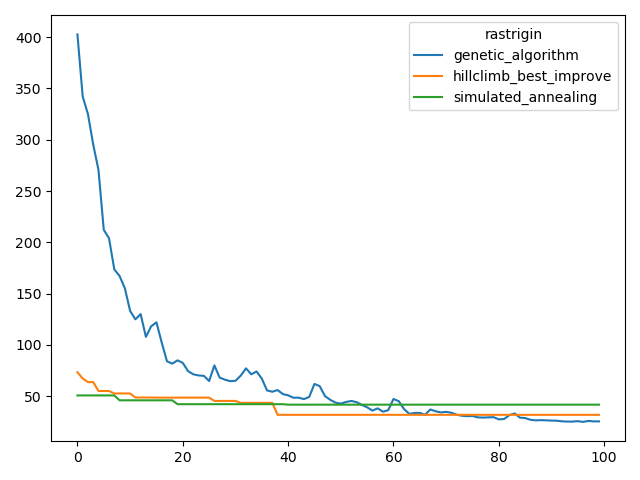
\includegraphics[width=0.75\linewidth]{rastrigin_graph.png}
    \caption{Rastrigin results graph}
    \label{fig7:b}
\end{figure}

As we begin interpreting the function graphs, we notice immediately that GA has a lot of instances where the best value for the next population is worse than the value of the previous. HC will always retain the best value, so it does not present this behaviour, but SA might create an instance where it would choose a weak solution to find one that is better. Still, SA then compares this to the current optimum so the bad values would be automatically ignored. Still, at some point one of the improvements might be caused by one of those bad choices and improve greately the global best. The reason why GA behaves differently is because in GA we do not have the concept of a global best, there is only the best in the population. When we move from one population to another we assume that the next one might be less optimal then the previous. \\

Also worth mentioning is the difference in starting points between GA and HC, SA. The last two begin from a better solution because they compare the values between iterations and reach a point that is either a local optimum or something else and return that. But for GA it simply starts with random chromosomes and starts optimising the population steadily, and does not update a global best. \\

We also notice that GA has in the end better results than the first two algorithms, and that is because HC and SA might - like in our instance - reach a point from which they cannot escape(or escape easily). GA is always modifying something, mutating and selecting, so the values always (or most of the time) change, so in the end it reaches a better solution.

\subsection{Schwefel}

Genetic Algorithm on Schwefel has produced the following results:

\begin{figure}[H]
\centerline{
\begin{tabular}{|c||c|c|c|c|c|c|c|}
\hline
\rowfont{\bfseries} Dim. & Mean & Max & Min & Median & MRT(sec.) & RT(min.) & StdDev \\ \hline
5 & 0.06637 & 0.20776 & 0.00000 & 0.10352 & 6.97189 & 3.48595 & 0.05644 \\
10 & 0.21616 & 0.31348 & 0.10547 & 0.20923 & 17.37879 & 8.68939 & 0.07493 \\
30 & 297.19870 & 506.46094 & 62.54395 & 310.91553 & 41.29582 & 20.64791 & 114.51190 \\
\hline
\end{tabular}
}
\end{figure}

Hillclimbing-best on Schwefel has produced the following results:

\begin{figure}[H]
\centerline{
\begin{tabular}{|c||c|c|c|c|c|c|c|}
\hline
\rowfont{\bfseries} Dim. & Mean & Max & Min & Median & MRT(sec.) & RT(min.) & StdDev \\ \hline
5 & 292.29132 & 387.63892 & 237.09009 & 237.09009 & 0.03423 & 0.01711 & 72.54864 \\
10 & 634.09524 & 981.04395 & 306.35840 & 627.99341 & 0.29534 & 0.14767 & 199.48108 \\
30 & 1973.12520 & 2515.98828 & 1482.08496 & 2016.91064 & 7.11674 & 3.55837 & 260.33367 \\
\hline
\end{tabular}
}
\end{figure}

Simulated Annealing on Schwefel has produced the following results:

\begin{figure}[H]
\centerline{
\begin{tabular}{|c||c|c|c|c|c|c|c|}
\hline
\rowfont{\bfseries} Dim. & Mean & Max & Min & Median & MRT(sec.) & RT(min.) & StdDev \\ \hline
5 & 264.56776 & 475.01636 & 27.87842 & 260.91876 & 3.00609 & 1.50304 & 104.52989 \\
10 & 707.11108 & 1101.05273 & 333.41235 & 696.53076 & 3.00621 & 1.50310 & 197.38461 \\
30 & 2773.79717 & 3372.21582 & 2042.97070 & 2846.76074 & 3.00604 & 1.50302 & 293.09082 \\
\hline
\end{tabular}
}
\end{figure}

The results have been computed on this graph:

\begin{figure}[H]
    \centering
    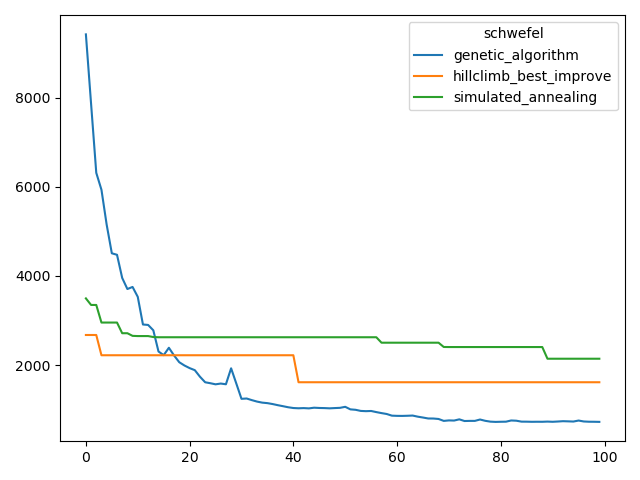
\includegraphics[width=0.75\linewidth]{schwefel_graph.png}
    \caption{Schwefel results graph}
    \label{fig7:b}
\end{figure}

In this graph we can observe that SA has a point around the $40^{nth}$ iteration where it breaks the local minima attraction pool and reaches a better solution. The Schwefel function is quite brutal when it comes to attraction basins, as we can see the large difference between the three sources of output.\\

\subsection{Sphere}

Genetic Algorithm on Sphere has produced the following results:

\begin{figure}[H]
\centerline{
\begin{tabular}{|c||c|c|c|c|c|c|c|}
\hline
\rowfont{\bfseries} Dim. & Mean & Max & Min & Median & MRT(sec.) & RT(min.) & StdDev \\ \hline
5 & 0.00000 & 0.00000 & 0.00000 & 0.00000 & 5.06041 & 2.53020 & 0.00000 \\
10 & 0.00000 & 0.00000 & 0.00000 & 0.00000 & 11.37833 & 5.68916 & 0.00000 \\
30 & 0.00006 & 0.00012 & 0.00004 & 0.00006 & 31.03870 & 15.51935 & 0.00002 \\
\hline
\end{tabular}
}
\end{figure}

Hillclimbing-best on Sphere has produced the following results:

\begin{figure}[H]
\centerline{
\begin{tabular}{|c||c|c|c|c|c|c|c|}
\hline
\rowfont{\bfseries} Dim. & Mean & Max & Min & Median & MRT(sec.) & RT(min.) & StdDev \\ \hline
5 & 0.00120 & 0.00120 & 0.00120 & 0.00120 & 0.00657 & 0.00329 & 0.00000 \\
10 & 0.01244 & 0.02840 & 0.00320 & 0.00320 & 0.03107 & 0.01554 & 0.01214 \\
30 & 0.10668 & 0.44200 & 0.01440 & 0.06220 & 0.95315 & 0.47657 & 0.10734 \\
\hline
\end{tabular}
}
\end{figure}

Simulated Annealing on Sphere has produced the following results:

\begin{figure}[H]
\centerline{
\begin{tabular}{|c||c|c|c|c|c|c|c|}
\hline
\rowfont{\bfseries} Dim. & Mean & Max & Min & Median & MRT(sec.) & RT(min.) & StdDev \\ \hline
5 & 0.41735 & 1.16289 & 0.04203 & 0.34125 & 3.00601 & 1.50301 & 0.25495 \\
10 & 1.33097 & 2.40128 & 0.59801 & 1.28658 & 3.00602 & 1.50301 & 0.50278 \\
30 & 5.24496 & 7.87754 & 2.37124 & 5.32371 & 3.00604 & 1.50302 & 1.19954 \\
\hline
\end{tabular}
}
\end{figure}

\begin{figure}[H]
    \centering
    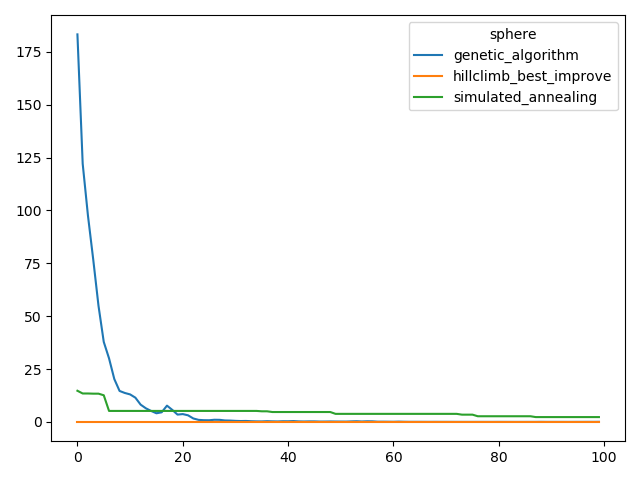
\includegraphics[width=0.75\linewidth]{sphere_graph.png}
    \caption{Sphere results graph}
    \label{fig7:b}
\end{figure}

In this instance we can see that on simpler functions the genetic algorithm improves quite fast, and also HC and SA often reach a good solution. In this case SA somehow found the optimal case but if it hadn't, we can expect the graph to resemble that of HC: steadily  improving, and sometimes jumping to a better solution.

\subsection{Rosenbrock}

Genetic algorithm on Rosenbrock has produced the following results:

\begin{figure}[H]
\centerline{
\begin{tabular}{|c||c|c|c|c|c|c|c|}
\hline
\rowfont{\bfseries} Dim. & Mean & Max & Min & Median & MRT(sec.) & RT(min.) & StdDev \\ \hline
5 & 2.28845 & 3.75156 & 0.22253 & 2.28204 & 5.34209 & 2.67105 & 1.04807 \\
10 & 7.51159 & 8.33795 & 4.35584 & 7.93529 & 12.23295 & 6.11648 & 0.88948 \\
30 & 28.24058 & 29.71366 & 25.24927 & 28.29572 & 31.88165 & 15.94082 & 0.79304 \\
\hline
\end{tabular}
}
\end{figure}

Hillclimbing-best on Rosenbrock has produced the following results:

\begin{figure}[H]
\centerline{
\begin{tabular}{|c||c|c|c|c|c|c|c|}
\hline
\rowfont{\bfseries} Dim. & Mean & Max & Min & Median & MRT(sec.) & RT(min.) & StdDev \\ \hline
5 & 134.72946 & 134.72946 & 134.72946 & 134.72946 & 0.00561 & 0.00281 & 0.00000 \\
10 & 94.63492 & 137.28891 & 20.58109 & 137.28891 & 0.04732 & 0.02366 & 56.06301 \\
30 & 172.91218 & 517.54858 & 30.81817 & 137.38277 & 1.22030 & 0.61015 & 128.69940 \\
\hline
\end{tabular}
}
\end{figure}

Simulated Annealing on Rosenbrock has produced the following results:

\begin{figure}[H]
\centerline{
\begin{tabular}{|c||c|c|c|c|c|c|c|}
\hline
\rowfont{\bfseries} Dim. & Mean & Max & Min & Median & MRT(sec.) & RT(sec.) & StdDev \\ \hline
5 & 58.39948 & 362.91174 & 3.50077 & 6.40541 & 3.00601 & 1.50301 & 90.77307 \\
10 & 257.32415 & 1946.52673 & 11.80267 & 130.76601 & 3.00602 & 1.50301 & 374.07534 \\
30 & 3671.87897 & 8397.09570 & 162.17835 & 3656.89038 & 3.00619 & 1.50309 & 2447.80553 \\
\hline
\end{tabular}
}
\end{figure}

The results have been computed on this graph:

\begin{figure}[H]
    \centering
    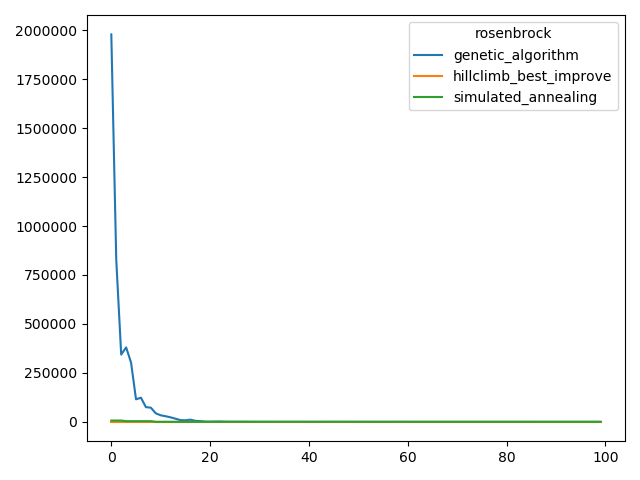
\includegraphics[width=0.75\linewidth]{rosenbrock_graph.png}
    \caption{Rosenbrock results graph}
    \label{fig7:b}
\end{figure}

Here on this graph GA starts from a ridiculously high value, but eventually reaches about 70, which is good, it means that our algorithm is able to move however much in order to get closer to a better solution. We can see that the same thing happens as in the case of Sphere functions: GA reacheas a good solution considerably faster than it would on a more complex function, and HC, SA can find an interestingly good solution in the first iterations.

\section{The Adaptive Genetic Algorithm}
Up until now the parameters/operators in GA were constant between runs and generations. But what if we can make them adapt to the current population or generation? This is the reason we built the AGA algorithm. This algorithm tries to optimize a genetic algorithm depending on its current population or the generation. \\
\par Also in this algorithm we will test an alternative binary representation, the Gray Code representation. This representation for bitstring chromosomes is known to alleviate the problems that appear with the Hamming distance between two chromosomes. This refers to the problem that between neighbouring values in the binary representation we have more than 1 bit to change, for instance between 7 and 8 we have to change 3 bits. For us to implement this new representation we only need to change our evaluation function: $$binary\_to\_decimal(bitstring) \longrightarrow binary\_to\_decimal(gray\_to\_binary(bitsring))$$ \\

The results on the 4 functions for AGA respectively are:\\

a) Rastrigin

\begin{figure}[H]
\centerline{
\begin{tabular}{|c||c|c|c|c|c|c|c|}
\hline
\rowfont{\bfseries} Dim. & Mean & Max & Min & Median & MRT(sec.) & RT(min.) & StdDev \\ \hline
5 & 0.00000 & 0.00000 & 0.00000 & 0.00000 & 5.16852 & 2.58426 & 0.00000 \\
10 & 0.00000 & 0.00000 & 0.00000 & 0.00000 & 9.95009 & 4.97505 & 0.00000 \\
30 & 0.09345 & 1.25995 & 0.01025 & 0.03804 & 29.62102 & 14.81051 & 0.22238 \\
\hline
\end{tabular}
}
\end{figure}

a) Schwefel

\begin{figure}[H]
\centerline{
\begin{tabular}{|c||c|c|c|c|c|c|c|}
\hline
\rowfont{\bfseries} Dim. & Mean & Max & Min & Median & MRT(sec.) & RT(min.) & StdDev \\ \hline
5 &  0.00002 & 0.00000 & 0.00024 & 0.00000 & 6.88254 & 3.44127 & 0.00006 \\
10 & 0.03838 & 0.20752 & 0.00000 & 0.00073 & 13.36661 & 6.68330 & 0.05649 \\
30 & 0.82165 & 1.21191 & 0.49707 & 0.81543 & 39.00801 & 19.50401 & 0.20661 \\
\hline
\end{tabular}
}
\end{figure}

a) Rosenbrock

\begin{figure}[H]
\centerline{
\begin{tabular}{|c||c|c|c|c|c|c|c|}
\hline
\rowfont{\bfseries} Dim. & Mean & Max & Min & Median & MRT(sec.) & RT(min.) & StdDev \\ \hline
5 & 0.88525 & 3.18561 & 0.00123 & 0.44674 & 5.59709 & 2.79855 & 0.90272 \\
10 & 4.90976 & 8.72149 & 0.23230 & 5.21653 & 10.32250 & 5.16125 & 2.20331 \\
30 & 27.68849 & 29.11929 & 24.43345 & 27.97688 & 30.30002 & 15.15001 & 1.18508 \\
\hline
\end{tabular}
}
\end{figure}

a) Sphere

\begin{figure}[H]
\centerline{
\begin{tabular}{|c||c|c|c|c|c|c|c|}
\hline
\rowfont{\bfseries} Dim. & Mean & Max & Min & Median & MRT(sec.) & RT(min.) & StdDev \\ \hline
5 & 0.00000 & 0.00000 & 0.00000 & 0.00000 & 5.31372 & 2.65686 & 0.00000 \\
10 & 0.00000 & 0.00000 & 0.00000 & 0.00000 & 9.84632 & 4.92316 & 0.00000 \\
30 & 0.00010 & 0.00016 & 0.00006 & 0.00009 & 29.12509 & 14.56255 & 0.00003 \\
\hline
\end{tabular}
}
\end{figure}

The new approach has proved to be a good choice, as results are now better. The implementation we used for it was the Gray Code decoding for our bitstrings and the following change: From 50 to 50 generations we test to see if the value is stuck in a local attraction basin. If so, we increase the mutation probability from 0.01 to 0.2 to reset the genes. We do this to allow our algorithm to search for other basins than the current one.

\begin{figure}[H]
  \begin{subfigure}[b]{0.5\linewidth}
    \centering
    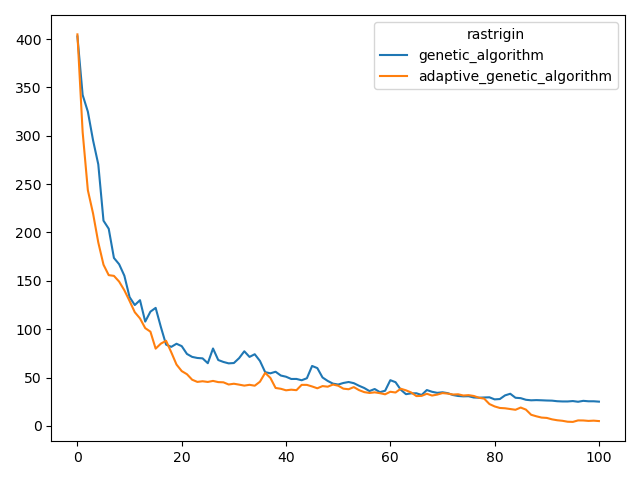
\includegraphics[width=0.75\linewidth]{age2p_rastrigin.png}
    \label{fig7:a}
    \vspace{4ex}
  \end{subfigure}%%
  \begin{subfigure}[b]{0.5\linewidth}
    \centering
    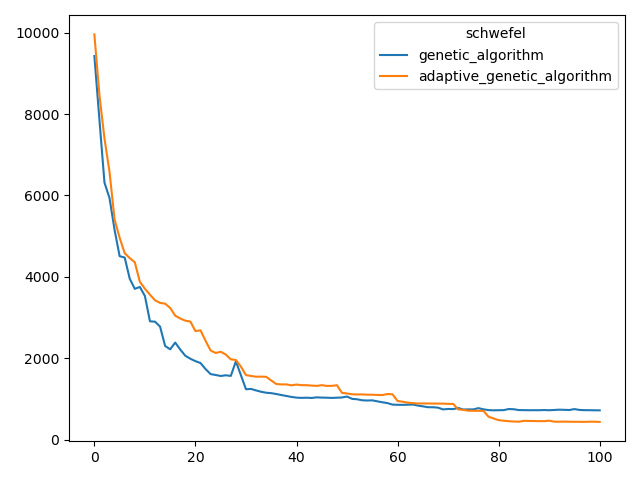
\includegraphics[width=0.75\linewidth]{age2p_schwefel.png}
    \label{fig7:b}
    \vspace{4ex}
  \end{subfigure}
\end{figure}
\begin{figure}[H]
  \begin{subfigure}[b]{0.5\linewidth}
    \centering
    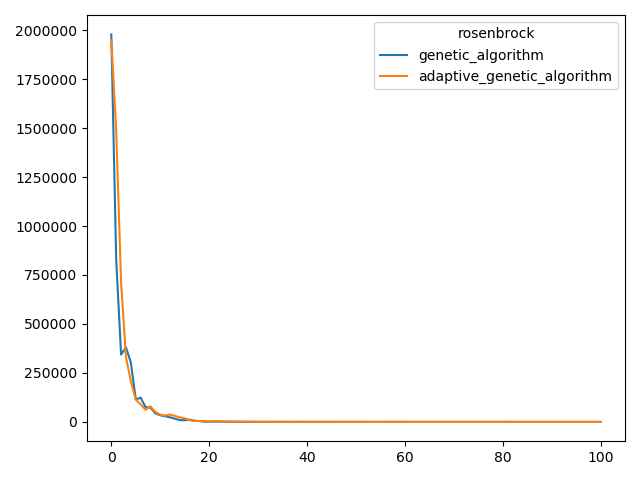
\includegraphics[width=0.75\linewidth]{age2p_rosenbrock.png}
    \label{fig7:c}
  \end{subfigure}%%
  \begin{subfigure}[b]{0.5\linewidth}
    \centering
    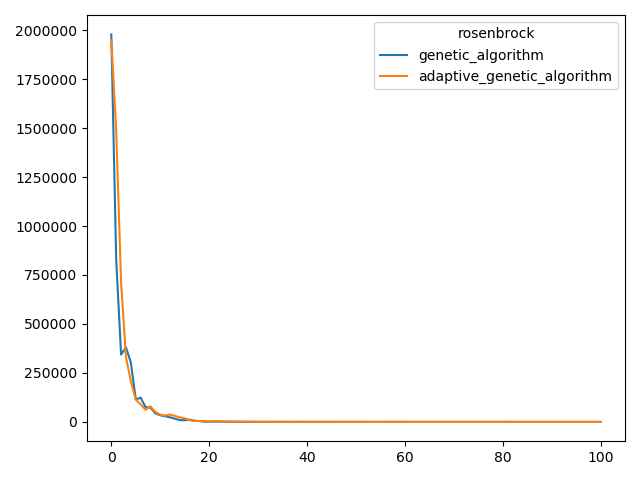
\includegraphics[width=0.75\linewidth]{age2p_sphere.png}
    \label{fig7:d}
  \end{subfigure}
  \caption{GA vs AGA}
  \label{fig7}
\end{figure}

The evolution in time for the two algorithms is quite resembling, and both of them show that in time the algorithms strive to provide better results. What is different though, is that we can notice on the graphs for Rastrigin and Schwefel certain bumps in the lineplot for the Adaptive Genetic Algorithm. This is likely caused by the mutation reset we mentioned earlier, thus making the population become tainted with unoptimal genes, that in time get ruled out again.

\section{Conclusions}
We have seen that using a Genetic Algorithm is a far better solution than HillClimbing and Simulated Annealing, even though out of the three GA is the slowest. What we learned from this is that in some problems, instead of comparing each individual with its successor in order to see which is the optimal path to take, it is beneficial that we start with a larger number of candidates that we test and try to adjust their form to one that is seemingly optimal. By doing so sistematically we are assured that (if we provide time) we will reach a good result. We have also learned how to improve our GA by making it adapt to its problem.\\
\par The Genetic Algorithm amazes us with its results and also because it is really intuitive. The fact that its inspiration comes from nature makes us think about how we can better combine this two domains and what interesting things we can discover by doing so.

\begin{thebibliography}

\bibitem{benchmarking}
BenchMarking Functions\\
\url{http://benchmarkfcns.xyz}
\bibitem{wikipedia}
Wikipedia\\Global optimization\\
\url{https://en.wikipedia.org/wiki/Global_optimization#Deterministic_methods}
\bibitem{Mating pool}
Mating pool\\
\url{https://en.wikipedia.org/wiki/Mating_pool}
\bibitem{Calin Crainiciun}
Calin Crainiciun - \\
For contributing with the ideea for the selection process to prioritise better solutions.
\bibitem{Gray1}
Code Gray\\
\url{https://en.wikipedia.org/wiki/Gray_code}
\bibitem{Gray2}
Code Gray vs Binary analysis\\
\url{https://www.umsl.edu/mathcs/about/People/Faculty/CezaryJanikow/untitled%20folder/An%20Alalysis.pdf}
\end{thebibliography}
\end{document}
